\documentclass[eng,openany]{mgr}
\usepackage{listings}
\usepackage[english]{babel}
\usepackage{graphicx}
\usepackage{hyperref}
\usepackage{tabularx,colortbl} 
\usepackage{rotating}
\usepackage[utf8]{inputenc} 
\setlength\parindent{24pt}
\usepackage[parfill]{parskip}
\usepackage[table,kernelfbox,hyperref]{xcolor}
\usepackage{fancyhdr}
\usepackage{gauss}
%\usepackage[colorinlistoftodos]{todonotes}

\hypersetup{colorlinks=true}
\hypersetup{xurlbordercolor=red!70!black}
\hypersetup{xlinkbordercolor=blue!70!black}
\hypersetup{linkcolor=blue!60!black}
\hypersetup{urlcolor=red!50!black}
\hypersetup{citecolor=green!30!black}
\rfoot{Page \thepage}
\renewcommand\lstlistlistingname{List of Listings}
\newcommand{\linia}{\rule{\linewidth}{0.4mm}}

\definecolor{listlightgray}{gray}{0.93}

\newcommand{\lstsetmylst} {
\lstset{frame = tb,
breaklines=true,
framerule = 0.25pt,
float,
fontadjust,
backgroundcolor={\color{listlightgray}},
basicstyle = {\ttfamily\footnotesize},
identifierstyle = {\ttfamily},
stringstyle = {\ttfamily},
showstringspaces = false,
showtabs = false,
numbers = left,
numbersep = 6pt,
tabsize = 4,
language=C,
floatplacement=!h
}
}

\newcommand{\lstsetatc} {
\lstset{frame = tb,
breaklines=true,
framerule = 0.25pt,
float,
fontadjust,
backgroundcolor={\color{listlightgray}},
basicstyle = {\ttfamily\footnotesize},
keywordstyle = {\ttfamily\color{listkeyword}\textbf},
identifierstyle = {\ttfamily},
commentstyle = {\ttfamily\color{listcomment}\textit},
stringstyle = {\ttfamily},
showstringspaces = false,
showtabs = false,
numbers = left,
numbersep = 6pt,
numberstyle={\ttfamily\color{listnumbers}},
tabsize = 4,
language=C,
floatplacement=!h
}
}

\newcommand{\lstsetatbashnum} {
\lstset{frame = tb,
breaklines=true,
framerule = 0.25pt,
aboveskip=2ex,
float,
fontadjust,
backgroundcolor={\color{listlightgray}},
basicstyle = {\ttfamily\footnotesize},
keywordstyle = {\ttfamily\color{listkeyword}\textbf},
identifierstyle = {\ttfamily},
commentstyle = {\ttfamily\color{listcomment}\textit},
stringstyle = {\ttfamily},
showstringspaces = false,
showtabs = false,
numbers = left,
numbersep = 6pt,
numberstyle={\ttfamily\color{listnumbers}},
tabsize = 4,
language=bash,
floatplacement=!h
}
}
\lstsetmylst
\author{Jaroslaw M. Szumega}
\title{}
\engtitle{}
\supervisor{Rafal Zdunek, D.Sc, K-4/W4}
\field{Electronics}
\specialisation{Advanced Applied Electronics}
\date{14.03.2017}
\begin{document}
\selectlanguage{english}
\maketitle

\newpage

\chapter{Solution to the given problems}
(Problems 1-6 are solved analytically, without using any of selected algorithms. But the results are checked.
Still - the analytical solution is made in Octave environment.)

\begin{figure}[h]
\centering
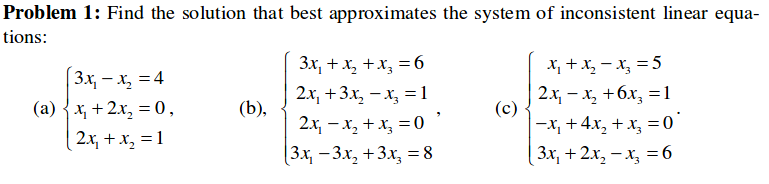
\includegraphics[width=0.9\linewidth]{screenshot001}
\label{fig:screenshot001}
\end{figure}

The set of equations can be solved by transforming it to matrix form and applying the gaussian elimination. We will get the matrix triangular form (upper triangular in this case - it will be solved with backsubstitution).

\begin{figure}[h]
\centering
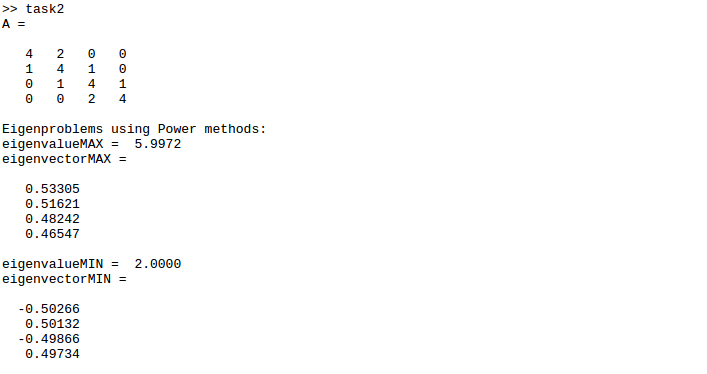
\includegraphics[width=0.7\linewidth]{screenshot002}
\label{fig:screenshot002}
\end{figure}

The matrices are presented above. The C matrix is a concatenation of matrix A and b - it will be used in elimination.\\
\begin{figure}
\centering
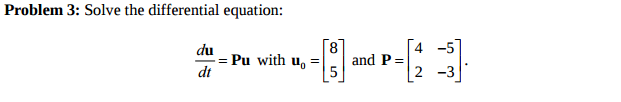
\includegraphics[width=0.3\linewidth]{screenshot004}
\caption{Step-by-step solution}
\label{fig:screenshot004}
\end{figure}

\newpage
\begin{figure}
\centering
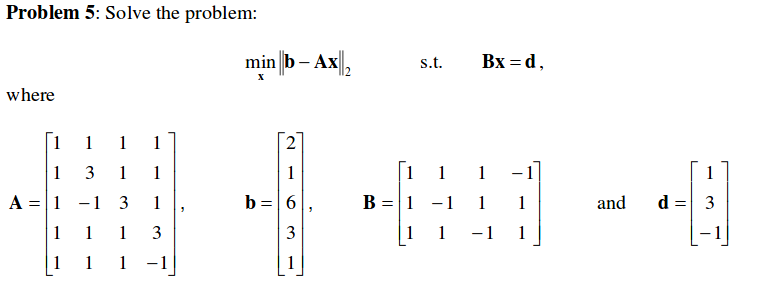
\includegraphics[width=0.7\linewidth]{screenshot005}
\caption{}
\label{fig:screenshot005}
\end{figure}

Just like in the previous problem - we will start from showing it in matrix form, and then start Gaussian elimination.

\begin{figure}[h]
\centering
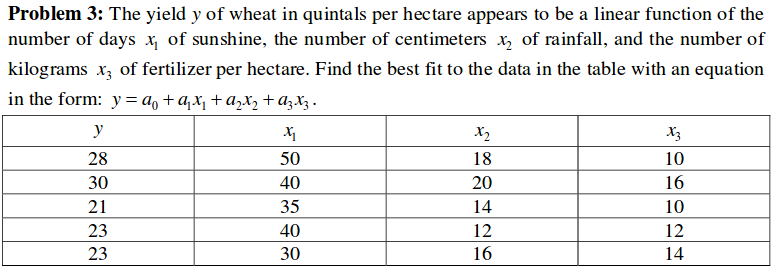
\includegraphics[width=0.3\linewidth]{screenshot006}
\caption{Solution in steps and solution by backsubstitution.}
\label{fig:screenshot006}
\end{figure}
\newpage

\begin{figure}[h]
\centering
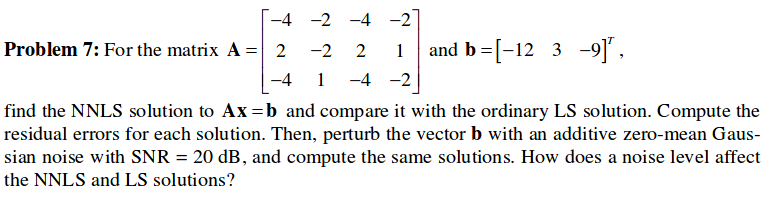
\includegraphics[width=0.7\linewidth]{screenshot007}
\label{fig:screenshot007}
\end{figure}

\begin{figure}[h]
\centering
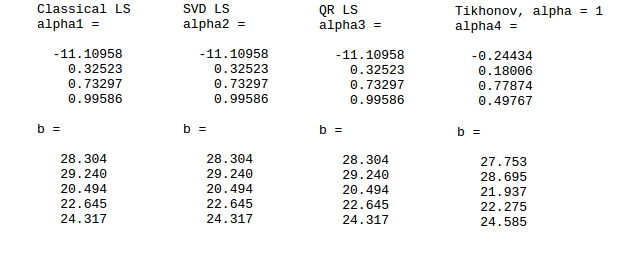
\includegraphics[width=0.8\linewidth]{screenshot008}
\caption{Computation with and without pivoting.}
\label{fig:screenshot008}
\end{figure}
The computed condition number of system matrix P:\\
cond(P)= 4.3916;
\newpage

\begin{figure}[h]
\centering
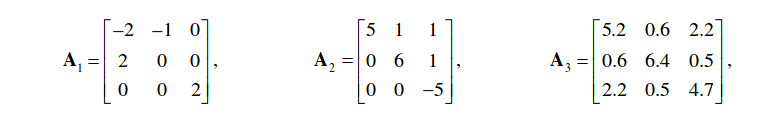
\includegraphics[width=0.7\linewidth]{screenshot009}
\label{fig:screenshot009}
\end{figure}

The solution obtained in matlab (step by step in Chapter 2).
\begin{figure}[h]
\centering
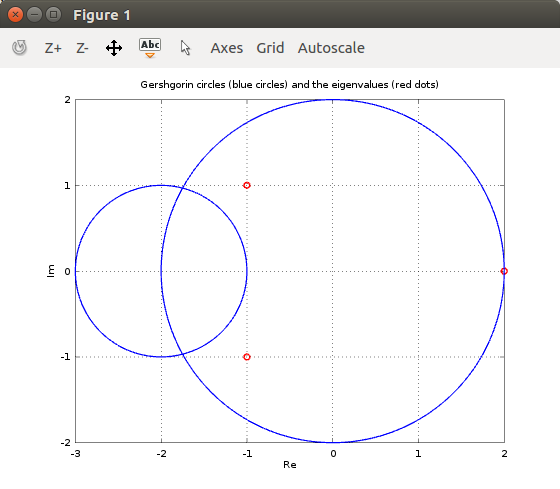
\includegraphics[width=0.7\linewidth]{screenshot010}
\label{fig:screenshot010}
\end{figure}

The condition number shows the stability between input and output. The one calculated here is rather big - that is the reson why after small perturbation the result changed so much.

\newpage
\begin{figure}[h]
\centering
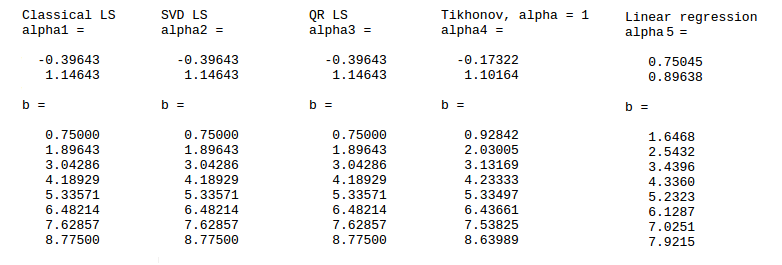
\includegraphics[width=0.7\linewidth]{screenshot011}
\label{fig:screenshot011}
\end{figure}
\begin{lstlisting}
A =
2   1   2
1   2   3
4   1   2

I =
1   0   0
0   1   0
0   0   1

System matrix:
C =
2   1   2   1   0   0
1   2   3   0   1   0
4   1   2   0   0   1

R2 - (a21)/(a11) R1
C =
2.00000   1.00000   2.00000   1.00000   0.00000   0.00000
0.00000   1.50000   2.00000  -0.50000   1.00000   0.00000
4.00000   1.00000   2.00000   0.00000   0.00000   1.00000

R3 - (a31)/(a11) R1
C =
2.00000   1.00000   2.00000   1.00000   0.00000   0.00000
0.00000   1.50000   2.00000  -0.50000   1.00000   0.00000
0.00000  -1.00000  -2.00000  -2.00000   0.00000   1.00000

R1 - (a12)/(a22) R2
C =
2.00000   0.00000   0.66667   1.33333  -0.66667   0.00000
0.00000   1.50000   2.00000  -0.50000   1.00000   0.00000
0.00000  -1.00000  -2.00000  -2.00000   0.00000   1.00000

R3 - (a32)/(a22) R2
C =
2.00000   0.00000   0.66667   1.33333  -0.66667   0.00000
0.00000   1.50000   2.00000  -0.50000   1.00000   0.00000
0.00000   0.00000  -0.66667  -2.33333   0.66667   1.00000

R1 - (a13)/(a33) R3
C =
2.00000   0.00000   0.00000  -1.00000   0.00000   1.00000
0.00000   1.50000   2.00000  -0.50000   1.00000   0.00000
0.00000   0.00000  -0.66667  -2.33333   0.66667   1.00000

R2 - (a23)/(a33) R3
C =
2.00000   0.00000   0.00000  -1.00000   0.00000   1.00000
0.00000   1.50000   0.00000  -7.50000   3.00000   3.00000
0.00000   0.00000  -0.66667  -2.33333   0.66667   1.00000


R1 / a11
C =

1.00000   0.00000   0.00000  -0.50000   0.00000   0.50000
0.00000   1.50000   0.00000  -7.50000   3.00000   3.00000
0.00000   0.00000  -0.66667  -2.33333   0.66667   1.00000

R2 / a22
C =

1.00000   0.00000   0.00000  -0.50000   0.00000   0.50000
0.00000   1.00000   0.00000  -5.00000   2.00000   2.00000
0.00000   0.00000  -0.66667  -2.33333   0.66667   1.00000

R3 / a33
C =

1.00000   0.00000   0.00000  -0.50000   0.00000   0.50000
0.00000   1.00000   0.00000  -5.00000   2.00000   2.00000
-0.00000  -0.00000   1.00000   3.50000  -1.00000  -1.50000

invA =

-0.50000   0.00000   0.50000
-5.00000   2.00000   2.00000
 3.50000  -1.00000  -1.50000

check with embedded function =

-0.50000   0.00000   0.50000
-5.00000   2.00000   2.00000
 3.50000  -1.00000  -1.50000
\end{lstlisting}
\newpage
\begin{figure}[h]
\centering
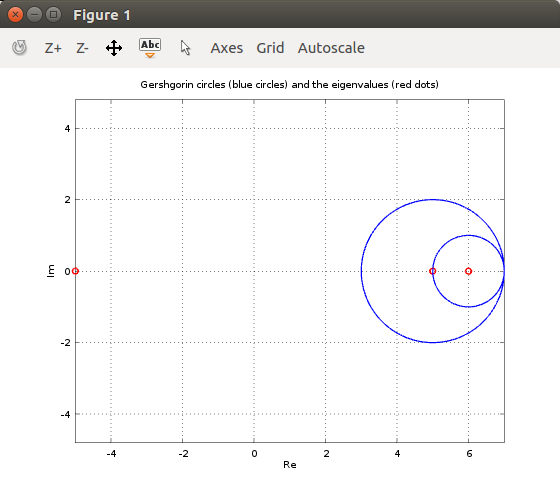
\includegraphics[width=0.7\linewidth]{screenshot012}
\end{figure}
\[
\begin{gmatrix}[p]
1 & 2 & 3 & 4 \\
-1 & 1 & 2 & 1 \\
0 & 2 & 1 & 3 \\
0 & 0 & 1 & 1
\end{gmatrix}
=
\begin{gmatrix}[p]
1 & 0 & 0 & 0 \\
L_{21} & 1 & 0 & 0 \\
L_{31} & L_{32} & 1 & 0 \\
L_{41} & L_{42} & L_{43} & 1
\end{gmatrix}
\begin{gmatrix}[p]
U_{11} & U_{12} & U_{13} & U_{14} \\
0 & U_{22} & U_{23} & U_{24} \\
0 & 0 & U_{33} & U_{24} \\
0 & 0 & 0 & U_{44}
\end{gmatrix}
\]


\begin{math}
 U_{11} = 1;  U_{12} = 2; U_{13} = 3; U_{14}=4
 \\\\
 L_{21}U_{11} = -1,\ so\  L_{21} = -1\\
 \\
 L_{21}U_{12} + U_{22} = 1,\ so\  U_{22} = 3\\
 L_{21}U_{13} + U_{23} = 2,\ so\  U_{23} = 5\\
 L_{21}U_{14} + U_{24} = 1,\ so\  U_{24} = 5\\ 
 \\
 L_{31}U_{11} = 0,\ so\  L_{31} = 0\\
 L_{31}U_{12} +L_{32}U_{22} = 2,\ so\  L_{32} = \frac{2}{3}\\
	\\ 
 L_{31}U_{13} + L_{32}U_{13} + U_{33} = 1,\ so\ U_{33} = -\frac{7}{3}\\
 L_{31}U_{14} + L_{32}U_{14} + U_{34} = 3,\ so\  U_{34} = -\frac{1}{3}\\
 \\
 L_{41} = 0 \\
 L_{42} = 0 \\
  L_{41}U_{13} + L_{42}U_{23} + L_{43}U_{33} = 1,\ so\ L_{43} = -\frac{3}{7}\\
  L_{43}U_{34} + L_{44}U_{44} = 1,\ so\  U_{34} = \frac{6}{7}\\
\end{math}
Solution:
\[
\begin{gmatrix}[p]
1 & 2 & 3 & 4 \\
-1 & 1 & 2 & 1 \\
0 & 2 & 1 & 3 \\
0 & 0 & 1 & 1
\end{gmatrix}
=
\begin{gmatrix}[p]
1 & 0 & 0 & 0 \\
-1 & 1 & 0 & 0 \\
0 & \frac{2}{3} & 1 & 0 \\
0 & 0 & -\frac{3}{7} & 1
\end{gmatrix}
\begin{gmatrix}[p]
1 & 2 & 3 & 4 \\
0 & 3 & 5 & 5 \\
0 & 0 & -\frac{7}{3} & -\frac{1}{3} \\
0 & 0 & 0 & \frac{6}{7}
\end{gmatrix}
\]
\begin{figure}[h]
\centering
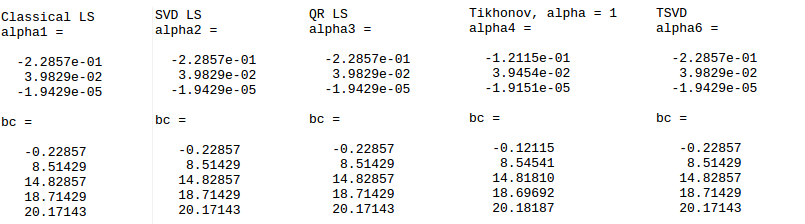
\includegraphics[width=0.4\linewidth]{screenshot013}
\label{fig:screenshot013}
\end{figure}
\newpage
The problems below are supposed to be solved using coded algorithms. Also some measurements related to execution time will be conducted.

To ensure proper timings, single measurement will check the elapsed time of a thousand of rounds for an algorithm. It will help to average the time, hence the additional timing like setting up environment etc. will be reduced. \\
That method is well known in algorithm's time complexity estimation.
\begin{figure}[h]
\centering
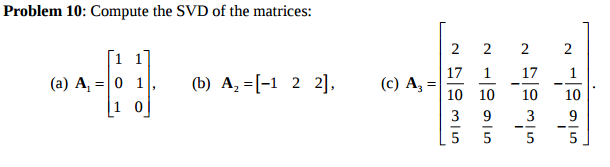
\includegraphics[width=0.7\linewidth]{screenshot014}
\label{fig:screenshot014}
\end{figure}
\begin{figure}[h]
\centering
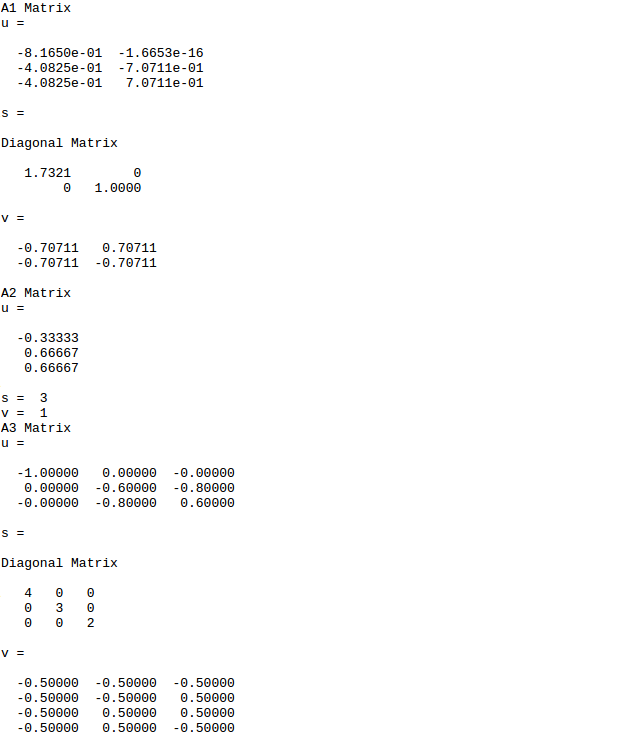
\includegraphics[width=0.7\linewidth]{screenshot015}
\label{fig:screenshot015}
\end{figure}

As the calculations show - the optimized embedded algorithm is almost 40x faster than the coded one.
\newpage
\begin{figure}[h]
\centering
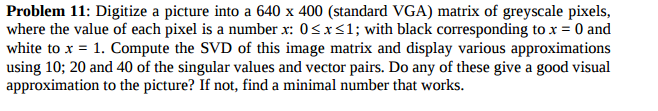
\includegraphics[width=0.7\linewidth]{screenshot016}

\label{fig:screenshot016}
\end{figure}
\begin{figure}[h]
\centering
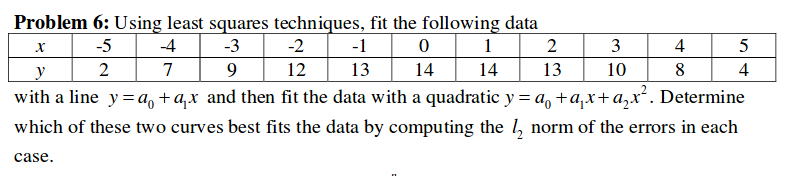
\includegraphics[width=0.7\linewidth]{screenshot017}
\label{fig:screenshot017}
\end{figure}
\newpage
\begin{figure}[h]
\centering
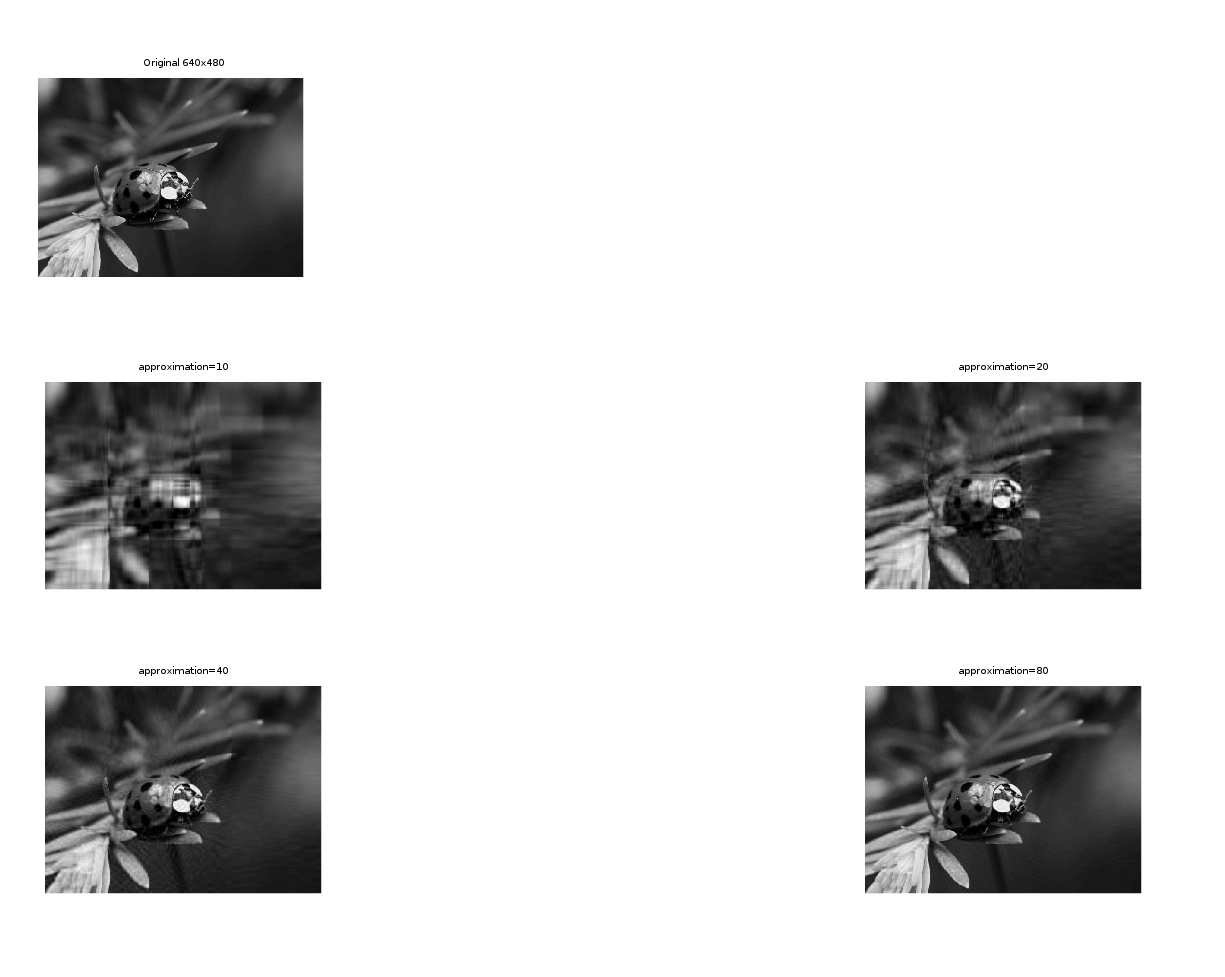
\includegraphics[width=0.7\linewidth]{screenshot018}
\end{figure}
Using Pascal matrix of order 100 for computation, the output was not very clear (Octave divided view among columns, rows etc.).
Therefore to see what is the result, the smaller matrices were used (matrices were checked for being positive definite).

\begin{figure}[h]
\centering
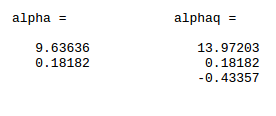
\includegraphics[width=0.7\linewidth]{screenshot019}
\caption{}
\end{figure}
The output looks like the upper triangular matrix derived from Pascal matrix, but the main diagonal are ones.
\newpage
\begin{figure}[h]
\centering
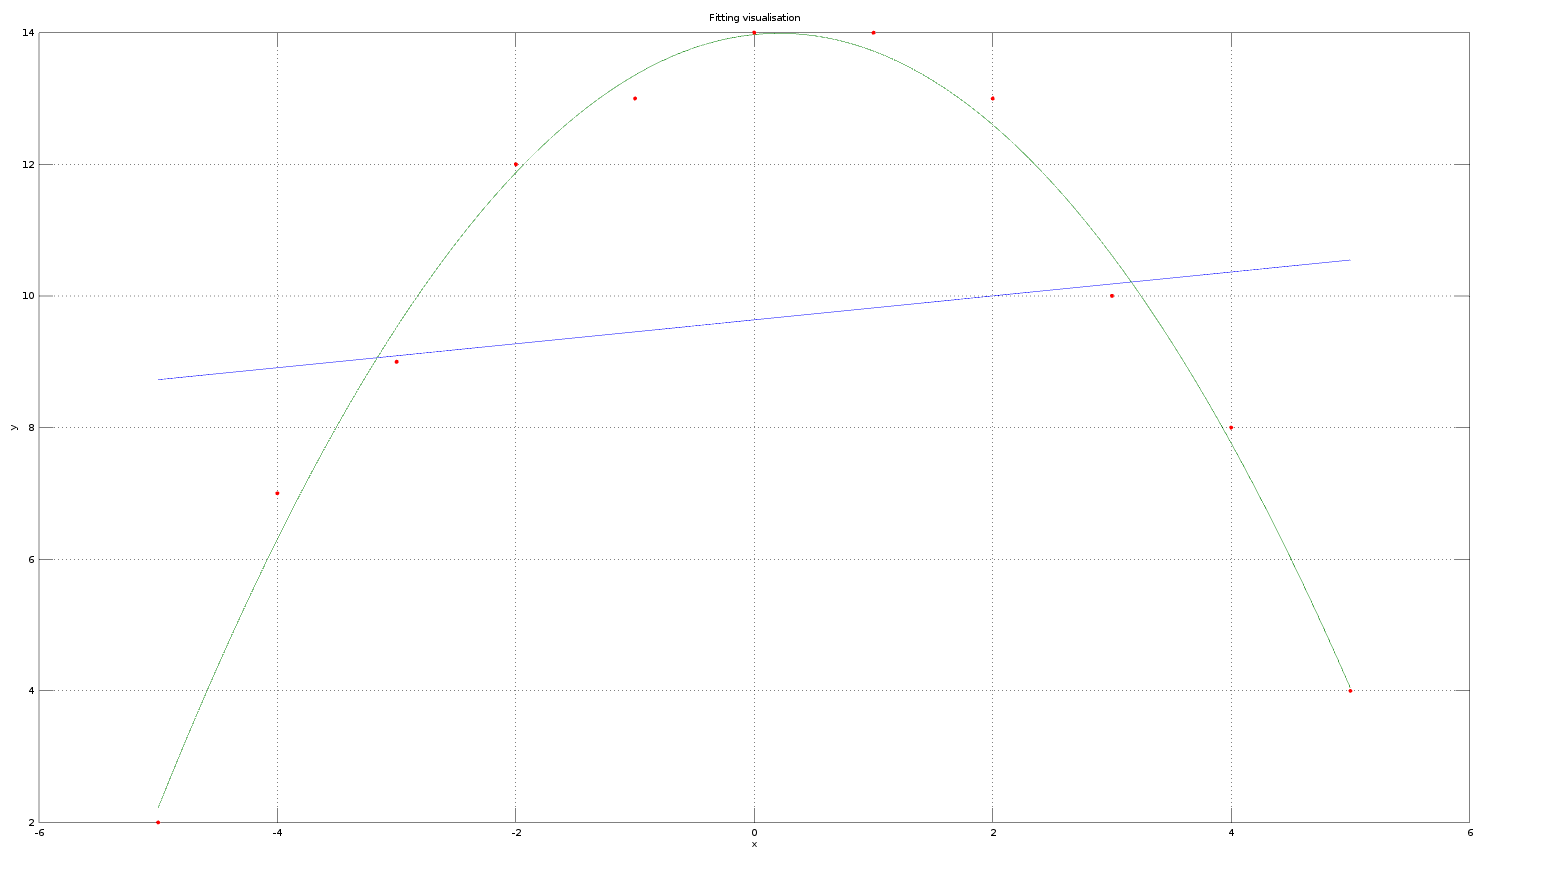
\includegraphics[width=0.7\linewidth]{screenshot020}
\label{fig:screenshot020}
\end{figure}

RREF (Row Reduced Echelon Form) can be obtained by using Gauss-Jordan elimination. That is the method used in the following case.
It is very easy to establish the matrix rank and free/basic variables only by taking a look at the final RREF result.
\begin{figure}[h]
\centering
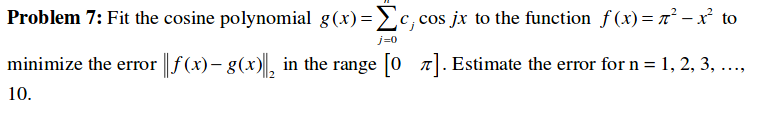
\includegraphics[width=0.7\linewidth]{screenshot021}
\label{fig:screenshot021}
\end{figure}

The first, third and fifth column are 'pivots column', so 
\begin{math}
x_{1}, x_{3}, x_{5} 
\end{math}
are basic variables, while non-pivots columns are second and fourth, therefore
\begin{math}
x_{2}, x_{4} 
\end{math}
are called "free variables".

To estimate the matrix rank, we take a look at the rows. There are 3 non-zero rows. \\
That way we know, the matrix rank is equal to 3.
\newpage
\begin{figure}[h]
\centering
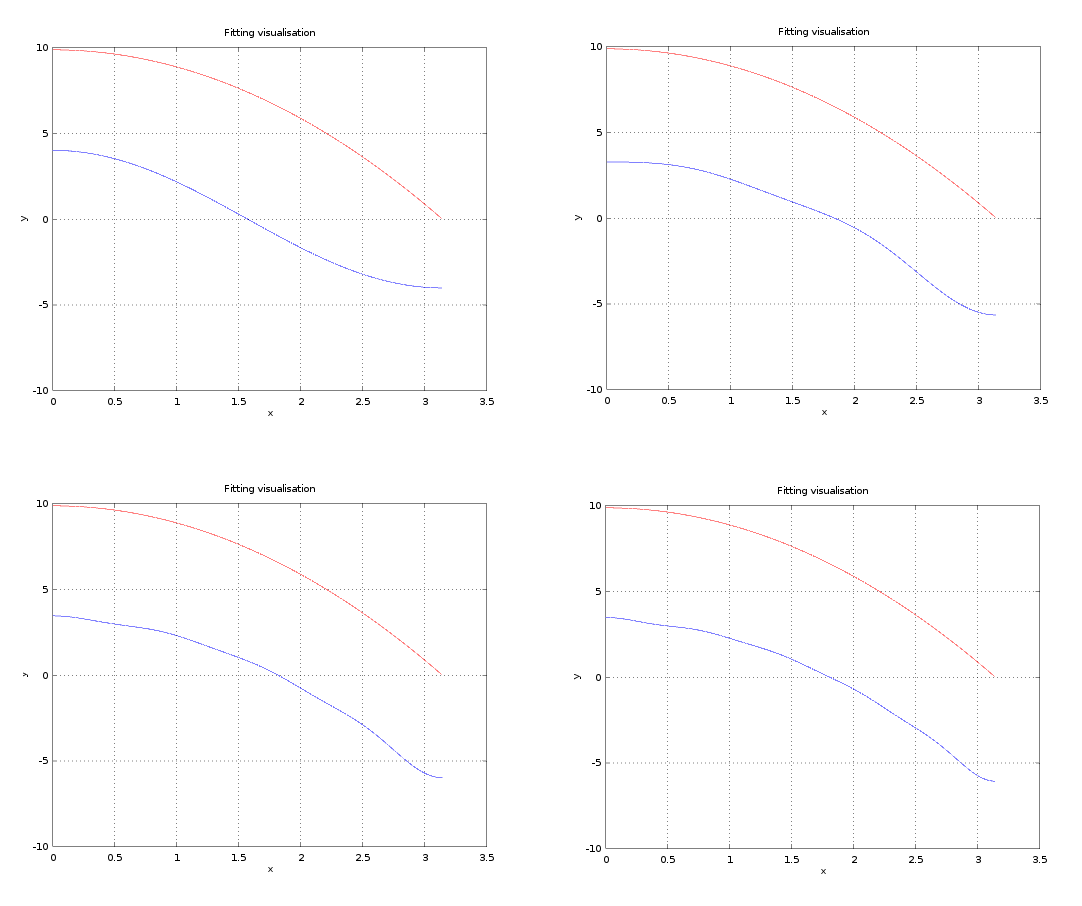
\includegraphics[width=0.7\linewidth]{screenshot022}
\label{fig:screenshot022}
\end{figure}
In this case, the LU factorization without pivoting does not work (there is Octave warning about division by zero).\\
Therefore the algorithm with pivoting shall be coded.

\newpage
\begin{figure}[h]
\centering
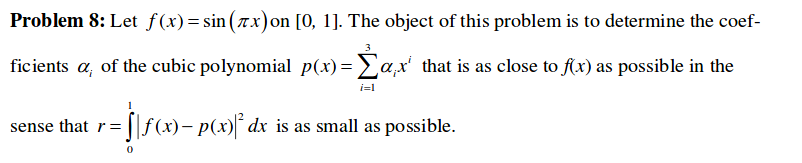
\includegraphics[width=0.7\linewidth]{screenshot023}
\label{fig:screenshot023}
\end{figure}

To solve this task, the QR by Givens rotations was used (mainly based on lecture notes).

\begin{figure}[h]
\centering
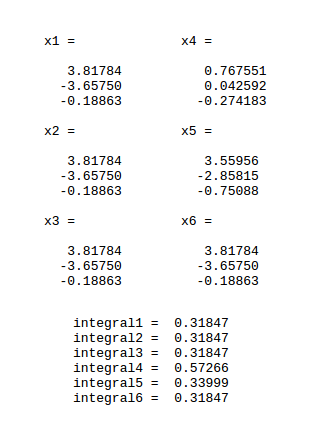
\includegraphics[width=0.6\linewidth]{screenshot024}
\caption{QR by Givens rotation along with checking by QR multiplying.}
\label{fig:screenshot024}
\end{figure}

There is a huge difference in computation time. The embedded version is almost 500x faster than the one written for lab purposes.

\newpage
\begin{figure}[h]
\centering
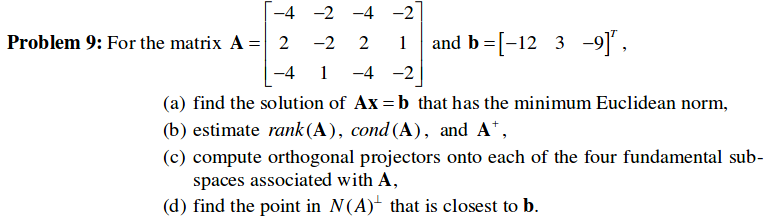
\includegraphics[width=0.7\linewidth]{screenshot025}
\label{fig:screenshot025}
\end{figure}

The solution to this problem requires two simple steps:
\begin{itemize}
	\item constructing set of formulas using Kirchoff's law for circuits that will be represented by matrix,
	\item solving the system matrix.
\end{itemize}

\[
\begin{gmatrix}[p]
 1 & 0 &  -1 & -1 &  0 &  0 &|\ 0 \\
 0 & 1 &   1 &  0 & -1 &  0 &|\ 0 \\
-1 & 0 &   0 &  0 &  1 &  1 &|\ 0 \\
 0 & 0 & -10 & 10 &  0 &  0 &| 10 \\
 0 & 0 &   0 & 10 &  0 & 10 &| 20 \\
 0 & 0 &   0 &  0 & 10 &-10 &| 10 \\
\end{gmatrix}
\]


\begin{figure}[h]
\centering
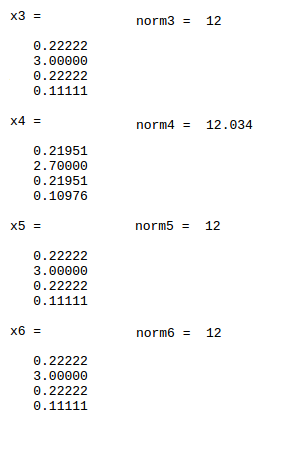
\includegraphics[width=0.7\linewidth]{screenshot026}
\label{fig:screenshot026}
\end{figure}

Looking at the output matrix it is easy to see, that:\\
\begin{math}
I_{1} = 2\\
I_{2} = 1\\
I_{3} = 0.5\\
I_{4} = 1.5\\
I_{5} = 1.5\\
I_{6} = 0.5\\
\end{math}

\chapter{Listings of solutions and algorithms}
\section{Octave files with problems solutions}
Problem no. 1
\begin{lstlisting}
A = [2 -1 0 0; -1 2 -1 0; 0 -1 2 -1; 0 0 -1 2];
b = [0; 0; 0; 5];
C = [A, b];

# basic operations to achieve upper triangular form
C
disp(['R1 <-> R2']);
C = exchange(C, 1, 2);

disp(['R2 = R2 + 2R1']);
C(2,:) = C(2,:) + 2*C(1,:);

disp(['R2 <-> R3']);
C = exchange(C,2,3);
disp(['R3 = R3 + 3R2']);
C(3,:) = C(3,:) + 3*C(2,:);

disp(['R3 <-> R4']);
C = exchange(C,3,4);
disp(['R4 = R4 + 4R3']);
C(4,:) = C(4,:) + 4*C(3,:);


#hand-made backsubstitution
x4 = z = C(4,5)/C(4,4);
x3 = w = (C(3,5) - C(3,4)*x4)/C(3,3);
x2 = v = (C(2,5) - C(2,3)*x3 - C(2,4)*x4)/C(2,2);
x1 = u = (C(1,5) - C(1,2)*x2 - C(1,3)*x3 - C(1,4)*x4)/C(1,1);

#and check with written gaussian elimination and backsubstitution
disp(['Check result']);
D = gaussian_elim([A,b]);
x = backsub(D)
\end{lstlisting}
\newpage
Problem no. 2
\begin{lstlisting}
disp(['Equations in of matrix form'])
A = [1 1 1; 1 1 2; 1 2 2]
b = [1;2;1]

disp(['Conacatenation of A and B'])
C = [A, b]

# piwot at 1,1
disp(['R2 = R2 - R1'])
C(2,:) = C(2,:) - C(1,:)
disp(['R3 = R3 - R1'])
C(3,:) = C(3,:) - C(1,:)

#element at 2,2 is zero, row interchange
disp(['R3 <-> R2'])
C = exchange(C,2,3)

x3 = C(3,4)/C(3,3)
x2 = (C(2,4) - C(2,3)*x3)/C(2,2)
x1 = (C(1,4) - C(1,2)*x2 - C(1,3)*x3)/C(1,1)
\end{lstlisting}
Problem no. 3
\begin{lstlisting}
A = [0.0001 1; 1 1 ]
b = [1;2]
P = [A, b]
NP = [A, b];
WP = [A, b];

disp(['Calculation without pivoting'])
disp([' '])
disp(['R2 - 1e-4*R1'])
NP(2,:) = NP(2,:) - 1e4*NP(1,:)

x2 = round(NP(2,3)/NP(2,2))
x1 = (NP(1,3) - NP(1,2))/NP(1,1)

disp([' '])
disp([' '])
disp(['And with pivoting'])
disp([' '])
disp(['R1<->R2'])
WP = exchange(WP,1,2)
disp(['R2 - 1e-4*R1'])
WP(2,:) = WP(2,:) - 1e-4*WP(1,:)


x2 = round(WP(2,3)/WP(2,2))
x1 = (WP(1,3) - WP(1,2))/WP(1,1)
\end{lstlisting}

\newpage
Problem no. 4
\begin{lstlisting}
A = [0.835 0.667; 0.333 0.266]
b = [0.168; 0.067]

disp(['System matrix:'])
C = [A b]

C(2,:) = C(2,:) - C(1,:) * (C(2,1)./C(1,1));
Cx2 = C(2,3)/C(2,2)
Cx1 = (C(1,3) - C(1,2)* Cx2)/C(1,1)

Ap = [0.835 0.667; 0.333 0.266];
b = [0.168; 0.066];

disp(['Small perturbation'])
D = [A b]

D(2,:) = D(2,:) - D(1,:) * (D(2,1)./D(1,1));
Dx2 = D(2,3)/D(2,2)
Dx1 = (D(1,3) - D(1,2)* Dx2)/D(1,1)

disp([' '])
disp(['Condition number of matrix'])
cond(C)

\end{lstlisting}
Problem no. 5
\begin{lstlisting}
A = [2 1 2; 1 2 3; 4 1 2]
I = [1 0 0; 0 1 0; 0 0 1]
disp(['System matrix:'])
C = [A I]

disp(['R2 - (a21)/(a11) R1'])
C(2,:) = C(2,:) - (C(2,1)/C(1,1)) * C(1,:)

disp(['R3 - (a31)/(a11) R1'])
C(3,:) = C(3,:) - (C(3,1)/C(1,1)) * C(1,:)

disp(['R1 - (a12)/(a22) R2'])
C(1,:) = C(1,:) - (C(1,2)/C(2,2)) * C(2,:)

disp(['R3 - (a32)/(a22) R2'])
C(3,:) = C(3,:) - (C(3,2)/C(2,2)) * C(2,:)

disp(['R1 - (a13)/(a33) R3'])
C(1,:) = C(1,:) - (C(1,3)/C(3,3)) * C(3,:)

disp(['R2 - (a23)/(a33) R3'])
C(2,:) = C(2,:) - (C(2,3)/C(3,3)) * C(3,:)

disp(['R1 / a11'])
C(1,:) = C(1,:)/C(1,1)
disp(['R2 / a22'])
C(2,:) = C(2,:)/C(2,2)
disp(['R3 / a33'])
C(3,:) = C(3,:)/C(3,3)
invC = C(:,4:6)
check = inv(A)
\end{lstlisting}
Problem no.7
\begin{lstlisting}
disp(['Init of Hilbert Matrix'])
H = hilb(5)

disp(['Programmed algorithm LU'])
[L, U] = lu_fac(H)

[n,n] = size(H);

disp(['Own determinant calculus'])
detH = 1;
for i = 1:n
detH = detH * U(i,i);
end
detH
disp(['Check with embedded function'])
det(H)

#+timing measurement
\end{lstlisting}

Problem no.8
\begin{lstlisting}
A = [1 -1 0 0; -1 2 -1 0; 0 -1 2 -1; 0 0 -1 2]


#is positive definite?
positivedefinite = all(eig(A) > 0)
#in this case G is upper triangular matrix
disp(['Cholesky factorization'])
G = cholesky_fac(A)

disp(['Inversion using coded Cholesky factorization'])
inv(G)*inv(G)'
disp(['Embedded inversion'])
inv(A)

#+timing measurement
\end{lstlisting}

Problem no.9
\begin{lstlisting}
A = pascal(100);
cholesky_fac(A);

B = pascal(5)
cholesky_fac(B)

C = pascal(10)
cholesky_fac(C)
\end{lstlisting}

Problem no.10
\begin{lstlisting}
A = [1 2 2 3 1; 2 4 4 6 2; 3 6 6 9 6; 1 2 4 5 3;]
RREF = alg_gjrref(A)
\end{lstlisting}

Problem no.11
\begin{lstlisting}
A = [1 3 3 2; 2 6 9 5; -1 -3 3 0]
B = lu_fac_pivot(A)
\end{lstlisting}

Problem no.12
\begin{lstlisting}
A = [0 -1 -3; 0 0 -2; 0 -2 1]

[Q, R] = QRgivens_lecture(A)

disp(['check by Q*R'])
Q*R



for i = 1:1000
[Q, R] = QRgivens_lecture(A);
end
toc
disp([' '])
disp([' '])
disp(['Embedded algorithm'])
tic
for i = 1:1000
[Q, R] = qr(A);
end
toc
\end{lstlisting}

Problem no.15
\begin{lstlisting}
 A = [1 0 -1 -1 0 0 0;
 0 1 1 0 -1 0 0;
 -1 0 0 0 1 1 0;
 0 0 -10 10 0   0  10;
 0 0 0  10  0   10 20;
 0 0  0  0  10 -10 10]
 
 disp(['Using gauss-jordan elimination'])
 alg_gjrref(A)
\end{lstlisting}
\newpage
\section{Coded selected algorithms}
Algorithm 1 - Gaussian elimination
\begin{lstlisting}
function [A] = gaussian_elim(A)

[n,m] = size(A);

for k = 1:n-1
#discussed on the lectre -> to avoid second loop, the 'rows' are used
rows = k+1:n;
A(rows, k) = A(rows,k)/A(k,k);
A(rows,rows) = A(rows,rows) - A(rows,k)*A(k,rows);
end
\end{lstlisting}

Algorithm 3 - Forward substitution
\begin{lstlisting}
function [b] = forwardsub(C)

[n,m] = size(C);

L = C(:,1:m-1);
b = C(:,m);

b(1) = b(1)/U(1,1);

for i = 2:n
b(i) = (b(i) - L(i, 1:i-1)*b(1:i-1))/L(i,i);

end
end
\end{lstlisting}

Algorithm 4 - Back substitution
\begin{lstlisting}
function [b] = backsub(C)

[n,m] = size(C);

U = C(:,1:m-1);
b = C(:,m);

b(n) = b(n)/U(n,n);

for i = n-1:-1:1
b(i) = (b(i) - U(i, i+1:n)*b(i+1:n))/U(i,i);

end
end
\end{lstlisting}
\newpage
Algorithm 5, 6 -- Gauss--Jordan, used also as RREF
\begin{lstlisting}
function [A] = alg_gjrref(A)

[n,m] = size(A);

j = 1;
for i = 1:n
#a
while(A(i:n,j) == 0)
j = j+1;

if(j>m)
return
endif
endwhile

#b
x = i;
while(A(i,j)==0)
x = x + 1;
if(x>n)
break;
endif
if(A(x,j)!=0)
temp = A(i,:);
A(i,:) = A(x, :);
A(x, :) =  temp;
break;
endif
endwhile

if(A(i,j)==0)
continue;
endif

#c
A(i,:) = A(i,:)/A(i,j);

#d
for k = 1:n
if( k == i)
continue;
endif
A(k,:) = A(k,:) - A(i,:)*A(k,j);
end 

end
end


\end{lstlisting}
\newpage
Algorithm 7 LU factorization
\begin{lstlisting}
function [L, U] = lu_fac(A)

[n, m] = size(A);

L = eye(n);
U = zeros(n,m);

for j = 1:n
if (j == 1)
v(j:n) = A(j:n,j);

else
#the elimination below won't work
#z = (A(1:j-1,j)) / (L(1:j-1, 1:j-1));

z = inv((L(1:j-1, 1:j-1))) * (A(1:j-1,j));
U(1:j-1, j) = z;

v(j:n) = A(j:n, j) - L(j:n, 1:j-1)*z;
endif

if(j<n)
L(j+1:n, j) = v(j+1:n) / v(j);
end
U(j,j) = v(j);

end
\end{lstlisting}
\newpage
Algorithm 8 -- LU factorization with pivoting
\begin{lstlisting}
function [L, U, p] = lu_fac_pivot(A)

[n, m] = size(A);

L = eye(n);
U = zeros(n,m);
p = zeros(n,n)

for j = 1:n
if (j == 1)
v(j:n) = A(j:n,j);

else
#the elimination below won't work??
#z = (A(1:j-1,j)) / (L(1:j-1, 1:j-1));

z = inv((L(1:j-1, 1:j-1))) * (A(1:j-1,j));
U(1:j-1, j) = z;

v(j:n) = A(j:n, j) - L(j:n, 1:j-1)*z;
endif

if(j<n)
[val, index] = max(v(j:n));
p(j) = index;
tempV = v(j);
v(j) = v(index);
v(index) = tempV;

tempA =  A(j,j+1:n)
A(j,j+1:n) = A(index, j+1:n);
A(index, j+1:n) = tempA;

L(j+1:n, j) = v(j+1:n) / v(j);

if(j>1)
tempL = L(j,1:j-1);
L(j,1:j-1) = L(index, 1:j-1);
L(index, 1:j-1) = tempL;
endif
endif
U(j,j) = v(j);

end
\end{lstlisting}
\newpage
Algorithm 10 -- Cholesky factorization
\begin{lstlisting}
function [G] = cholesky_fac(A)

G = A;
[n,k] = size(G);

for j = 1:n
if (j>1)
G(j:n,j) = G(j:n,j) - G(j:n,1:j-1)*G(j,1:j-1)';
end
G(j:n,j) = G(j:n,j)/sqrt(G(j,j));
end

#at the end -> eliminate what has left from A matrix when i>j
for i = 1:n
for j = 1:k

if(i>j)
G(i,j) = 0;

end
end


end
\end{lstlisting}

Algorithm 12 -- QR by Givens rotation
\begin{lstlisting}
function [ Q,R ] = QRgivens_lecture( A )

[n, n] =size(A);
Q=eye(n);
R=A;
for j=1:n
for i=n:(-1):j+1
x=R(:,j);
if norm([x(i-1),x(i)])>0

# calculate givens c and s
c=x(i-1)/norm([x(i-1),x(i)]);
s=-x(i)/norm([x(i-1),x(i)]);

G=eye(n);

#update
G([i-1,i],[i-1,i])=[c,s;-s,c];

R=G'*R;
Q=Q*G;
end

end
end

\end{lstlisting}
\begin{thebibliography}{8}
\addcontentsline{toc}{chapter}{Bibliography}
%\addcontentsline{toc}{section}{Literatura}
\bibitem{bjorck}
Björck, Åke. Numerical methods for least squares problems. Society for Industrial and Applied Mathematics, 1996.
\bibitem{golub}
Golub, Gene H., and Charles F. Van Loan. "Matrix computations, 3rd." (1996).
\bibitem{www}
Transforming a matrix to reduced row echelon form, http://www.di-mgt.com.au/matrixtransform.html
\bibitem{zdunek}
Zdunek R., Numerical Methods - lecture slides.
\end{thebibliography}

\end{document}

